\makeatletter

\newcommand{\sectionFormated}[1]
{
\vspace{10mm}
\section{#1}
\vspace{3mm}
}

\newcommand{\subsectionFormated}[1]
{
\vspace{10mm}
\subsection{#1}
\vspace{3mm}
}

\makeatother

\headheight = 2cm
\sectionFormated{Описание рабочей среды}

\begin{tabular}{l}
{\normalize
    - Модель процессора:\\
    - Число ядер:\\
    - Архитектура:\\
    - ОС:\\
    - RAM объем:\\
    - RAM тип:\\
    - Среда разработки:\\
    - Компилятор:\\
    - Версия OpenMP:\\
}
\end{tabular}
\hfill
\begin{tabular}{l}
{\normalize
    Intel Core i3-10110U CPU @ 2.10GHz\\
    4\\
    x86-64\\
    Linux, дистрибутив Ubuntu v20.04\\
    2x8192 MB\\
    DDR4\\
    Visual Studio Code\\
    gcc v9.4.0\\
    201511\\
}
\end{tabular}

\sectionFormated{Анализ приведенного алгоритма}

В задании лабораторной работы приведена программа, осуществляющая поиск заданного элемента в массиве.

Основное отличие от задания лабораторной работы 1 заключается в том, что при первом нахождение заданного элемента продолжать поиск не требуется.

\subsectionFormated{Блоксхема алгоритма}
\begin{center}
    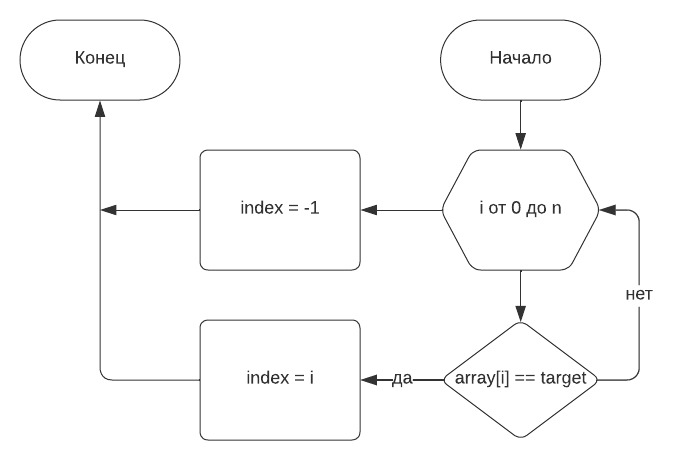
\includegraphics[scale=1.4]{images/block_diagram.jpeg}
\end{center}

\newpage

\subsectionFormated{Описание используемых директив OpenMP}

\verb|parallel| - определяет параллельную область, которая представляет собой код, который будет выполняться несколькими потоками параллельно. Директива \verb|parallel| была объявлена со следующими атрибутами:

\vspace{1mm}
\begin{itemize}
\setlength{\itemsep}{10pt}
    \item \verb|num_threads()| - задаёт количество потоков в параллельном блоке (по умолчанию \verb|parallel| использует все потоки);
%    \item \verb|reduction()| - определяет переменную, являющихся приватными для каждого потока, при выходе которые подвергаются операции редукции;
    \item \verb|shared()| - объявляет, что переменные должны быть общими между всеми потоками;
%    \item \verb|default()| - задаёт стандартное поведение при встрече неинициализированной внутри потока переменной.
\end{itemize}
\vspace{3mm}

\verb|for| - разделяет работу цикла между потоками (без неё каждый поток обрабатывал бы весь массив).\\

Действие директивы \verb|parallel| распространяется на следующий блок программного кода:

\begin{lstlisting}[
    language=C,
    belowskip=-0.8 \baselineskip
    ]
#pragma omp for
for(int i = 0; i < count; i++) {
    if (flag) continue;

    if(array[i] == target) {
        #pragma omp critical
        {
            index = i;
            flag = true;
        }
    }
}
\end{lstlisting}

\vspace{10mm}
В свою очередь директива \verb|for| действует на следующую строку:

\begin{lstlisting}[
    language=C,
    belowskip=-0.8 \baselineskip
    ]
for(int i = 0; i < count; i++)
\end{lstlisting}

\vspace{10mm}
\verb|critical| - определяет раздел кода, который должен выполняться одним потоком за раз.

\newpage

\subsectionFormated{Описание работы алгоритма}

Дерективой \verb|parallel| объявляется блок кода, который будет исполняться параллельно. Далее внутри \verb|for| потоки распередяют меду собой итерации цикла. Каждый поток ищет элемент равный заданному. При нахождении такого элемента внутри \verb|critical| переменной \verb|index| присваевается найденное значение индекса. После этого потоки перестают искать элемент, пропуская итерации цикла с помощью \verb|continue|.

\sectionFormated{Анализ временных характеристик последовательного алгоритма}

\subsectionFormated{Описание эксперимента}

\begin{itemize}
    \item Эксперименты проводились на шести типах массивов

\begin{description}
    \item[mode 0:] Заданный элемент находится на первой позиции
    \item[mode 1:] Заданный элемент находится в центре массива
    \item[mode 2:] Заданный элемент находится на последней позиции
    \item[mode 3:] Рандомный массив
    \item[mode 4:] Все элементы подходят
    \item[mode 5:] Ни один элемент не подходит
\end{description}

    \item Измеряется время работы алгоритма на 1\hspace{1mm}000 различных массивах длиной 10\hspace{1mm}000\hspace{1mm}000 элементов. Находится среднее значение;
\end{itemize}

\subsectionFormated{Экспериментальные показатели}
\begin{itemize}
    \item Среднее время работы последовательного алгоритма

\begin{description}
    \item[mode 0:] \verb|O(1)| 1.7 * $10^{-7}$ [с]
    \item[mode 1:] \verb|O(n)| 0.01300013 [с]
    \item[mode 2:] \verb|O(n)| 0.02465431 [с]
    \item[mode 3:] \verb|O(n)| 0.01212091 [с]
    \item[mode 4:] \verb|O(1)| 2.3 * $10^{-7}$ [с]
    \item[mode 5:] \verb|O(n)| 0.0260270390 [с]
\end{description}
\end{itemize}

\newpage

\raggedbottom \sectionFormated{Анализ временных характеристик параллельного алгоритма}

\subsectionFormated{Описание эксперимента}
\begin{itemize}
    \item Эксперименты проводились на шести типах массивов

\begin{description}
    \item[mode 0:] Заданный элемент находится на первой позиции
    \item[mode 1:] Заданный элемент находится в центре массива
    \item[mode 2:] Заданный элемент находится на последней позиции
    \item[mode 3:] Рандомный массив
    \item[mode 4:] Все элементы подходят
    \item[mode 5:] Ни один элемент не подходит
\end{description}

    \item измеряется время работы алгоритма для одного и того же массива, но на разном числе потоков: от 1 до 10;
    \item измерения производятся для 1\hspace{1mm}000 различных массивов, размер массива 10\hspace{1mm}000\hspace{1mm}000 элементов.
\end{itemize}

\newpage

\subsectionFormated{Результаты измерений}

Следующие таблицы содержат полученные в результате эксперимента данные: среднее время работы для различного числа потоков и конфигураций массивов.

\vspace{2cm}

\begin{center}
\begin{tabular}{ccc} 

\csvautotabular{plots_data/avg_0.csv} &
\csvautotabular{plots_data/avg_1.csv} &
\csvautotabular{plots_data/avg_2.csv}
    
\end{tabular}
\end{center}

\begin{center}
\begin{tabular}{ccc} 

\csvautotabular{plots_data/avg_3.csv} &
\csvautotabular{plots_data/avg_4.csv} &
\csvautotabular{plots_data/avg_5.csv}
    
\end{tabular}
\end{center}

\newpage
\subsectionFormated{Графики}

\begin{adjustwidth}{-1cm}{}
\subsectionFormated{1. Заданный элемент на первой позиции (mode 0)}
\end{adjustwidth}
\begin{tikzpicture}
\begin{axis}[
    title style={at={(0.5,1.12)},anchor=north,yshift=-0.1},
    title={\textbf{Зависимость времени работы от числа потоков}},
    xlabel={Число потоков},
    ylabel={Среднее время работы [с]},
    xmin=1, xmax=10,
    ymin=0, ymax=0.02,
    xtick distance = 1,
    legend pos=north east,
    xmajorgrids=true,
    grid style={dotted, gray},
    ymajorgrids=true,
    restrict y to domain=-10:10,
    ]

\addplot table[
    blue,
    mark=square,
    col sep=comma
] {plots_data/avg_0.csv};
\addlegendentry{Экспериментальные данные}
    
\addplot[
    thin,
    dashed,
    samples=4,
    red,
    domain={1:4}
] {0.012916 / x};

\addplot[
    thin,
    dashed,
    samples=8,
    red,
    domain={4:10}
] {0.012916 / 4};
\addlegendentry{Теоретические значения}
    
\end{axis}
\end{tikzpicture}\\

\newpage

\begin{figure}
\begin{adjustwidth}{-2cm}{}
\begin{center}
\begin{tabular}{cc} 

\begin{tikzpicture}[scale=0.65]
\begin{axis}[
    title style={at={(0.5,1.12)},anchor=north,yshift=-0.1},
    title={\textbf{Зависимость ускорения от числа потоков}},
    xlabel={Число потоков},
    ylabel={Ускорение},
    xmin=1, xmax=10,
    ymin=0, ymax=6,
    xtick distance = 1,
    legend pos=north east,
    xmajorgrids=true,
    ymajorgrids=true,
    grid style={dotted, gray},
    restrict y to domain=-10:10,
]

\addplot table[
    blue,
    mark=square,
    col sep=comma
] {plots_data/spu_0.csv};
\addlegendentry{Экспериментальные данные}

\addplot[
    thin,
    dashed,
    red,
    domain={1:4}
] {x};

\addplot[
    thin,
    dashed,
    red,
    domain={4:10}
] {4};
\addlegendentry{Теоретические значения}

\end{axis}
\end{tikzpicture}

&

\begin{tikzpicture}[scale=0.65]
\begin{axis} [
    title style={at={(0.5,1.12)},anchor=north,yshift=-0.1},
    title={\textbf{Зависимость эффективности от числа потоков}},
    xlabel={Число потоков},
    ylabel={Эффективность},
    xmin=1, xmax=10,
    ymin=0, ymax=1.3,
    xtick distance = 1,
    legend pos=north east,
    xmajorgrids=true,
    ymajorgrids=true,
    grid style={dotted, gray},
    restrict y to domain=-10:10,
]

\addplot table[
    blue,
    mark=square,
    col sep=comma
] {plots_data/eff_0.csv};
\addlegendentry{Экспериментальные данные}

\addplot[
    thin,
    dashed,
    red,
    domain={1:4}
] {1};

\addplot[
    thin,
    dashed,
    red,
    samples=12,
    domain={4:10}
] {4 / x};
\addlegendentry{Теоретические значения}

\end{axis}
\end{tikzpicture}
    
\end{tabular}
\end{center}
\end{adjustwidth}
\end{figure}

\newpage

\begin{adjustwidth}{-1cm}{}
\subsectionFormated{2. Заданный элемент в центре (mode 1)}
\end{adjustwidth}
\begin{tikzpicture}
\begin{axis}[
    title style={at={(0.5,1.12)},anchor=north,yshift=-0.1},
    title={\textbf{Зависимость времени работы от числа потоков}},
    xlabel={Число потоков},
    ylabel={Среднее время работы [с]},
    xmin=1, xmax=10,
    ymin=0, ymax=0.02,
    xtick distance = 1,
    legend pos=north east,
    xmajorgrids=true,
    grid style={dotted, gray},
    ymajorgrids=true,
    restrict y to domain=-10:10,
    ]

\addplot table[
    blue,
    mark=square,
    col sep=comma
] {plots_data/avg_1.csv};
\addlegendentry{Экспериментальные данные}
    
\addplot[
    thin,
    dashed,
    samples=4,
    red,
    domain={1:4}
] {0.017338 / x};

\addplot[
    thin,
    dashed,
    samples=8,
    red,
    domain={4:10}
] {0.017338 / 4};
\addlegendentry{Теоретические значения}
    
\end{axis}
\end{tikzpicture}\\

\newpage

\begin{figure}
\begin{adjustwidth}{-2cm}{}
\begin{center}
\begin{tabular}{cc} 

\begin{tikzpicture}[scale=0.65]
\begin{axis}[
    title style={at={(0.5,1.12)},anchor=north,yshift=-0.1},
    title={\textbf{Зависимость ускорения от числа потоков}},
    xlabel={Число потоков},
    ylabel={Ускорение},
    xmin=1, xmax=10,
    ymin=0, ymax=6,
    xtick distance = 1,
    legend pos=north east,
    xmajorgrids=true,
    ymajorgrids=true,
    grid style={dotted, gray},
    restrict y to domain=-10:10,
]

\addplot table[
    blue,
    mark=square,
    col sep=comma
] {plots_data/spu_1.csv};
\addlegendentry{Экспериментальные данные}

\addplot[
    thin,
    dashed,
    red,
    domain={1:4}
] {x};

\addplot[
    thin,
    dashed,
    red,
    domain={4:10}
] {4};
\addlegendentry{Теоретические значения}

\end{axis}
\end{tikzpicture}

&

\begin{tikzpicture}[scale=0.65]
\begin{axis} [
    title style={at={(0.5,1.12)},anchor=north,yshift=-0.1},
    title={\textbf{Зависимость эффективности от числа потоков}},
    xlabel={Число потоков},
    ylabel={Эффективность},
    xmin=1, xmax=10,
    ymin=0, ymax=1.3,
    xtick distance = 1,
    legend pos=north east,
    xmajorgrids=true,
    ymajorgrids=true,
    grid style={dotted, gray},
    restrict y to domain=-10:10,
]

\addplot table[
    blue,
    mark=square,
    col sep=comma
] {plots_data/eff_1.csv};
\addlegendentry{Экспериментальные данные}

\addplot[
    thin,
    dashed,
    red,
    domain={1:4}
] {1};

\addplot[
    thin,
    dashed,
    red,
    samples=12,
    domain={4:10}
] {4 / x};
\addlegendentry{Теоретические значения}

\end{axis}
\end{tikzpicture}
    
\end{tabular}
\end{center}
\end{adjustwidth}
\end{figure}

\newpage

\begin{adjustwidth}{-1cm}{}
\subsectionFormated{3. Заданный элемент на последней позиции (mode 2)}
\end{adjustwidth}
\begin{figure}[h]
\begin{adjustwidth}{-2cm}{}

\begin{center}
\begin{tikzpicture}[scale=0.95]
\begin{axis}[
    title style={at={(0.5,1.12)},anchor=north,yshift=-0.1},
    title={\textbf{Зависимость времени работы от числа потоков}},
    xlabel={Число потоков},
    ylabel={Среднее время работы [с]},
    xmin=1, xmax=10,
    ymin=0, ymax=0.03,
    xtick distance = 1,
    legend pos=north east,
    xmajorgrids=true,
    grid style={dotted, gray},
    ymajorgrids=true,
    restrict y to domain=-10:10,
    ]

\addplot table[
    blue,
    mark=square,
    col sep=comma
] {plots_data/avg_2.csv};
\addlegendentry{Экспериментальные данные}
    
\addplot[
    thin,
    dashed,
    samples=4,
    red,
    domain={1:4}
] {0.025239 / x};

\addplot[
    thin,
    dashed,
    samples=8,
    red,
    domain={4:10}
] {0.025239 / 4};
\addlegendentry{Теоретические значения}
    
\end{axis}
\end{tikzpicture}\\
\end{center}

\begin{center}
\begin{tabular}{cc} 

\begin{tikzpicture}[scale=0.65]
\begin{axis}[
    title style={at={(0.5,1.12)},anchor=north,yshift=-0.1},
    title={\textbf{Зависимость ускорения от числа потоков}},
    xlabel={Число потоков},
    ylabel={Ускорение},
    xmin=1, xmax=10,
    ymin=0, ymax=6,
    xtick distance = 1,
    legend pos=north east,
    xmajorgrids=true,
    ymajorgrids=true,
    grid style={dotted, gray},
    restrict y to domain=-10:10,
]

\addplot table[
    blue,
    mark=square,
    col sep=comma
] {plots_data/spu_2.csv};
\addlegendentry{Экспериментальные данные}

\addplot[
    thin,
    dashed,
    red,
    domain={1:4}
] {x};

\addplot[
    thin,
    dashed,
    red,
    domain={4:10}
] {4};
\addlegendentry{Теоретические значения}

\end{axis}
\end{tikzpicture}

&

\begin{tikzpicture}[scale=0.65]
\begin{axis} [
    title style={at={(0.5,1.12)},anchor=north,yshift=-0.1},
    title={\textbf{Зависимость эффективности от числа потоков}},
    xlabel={Число потоков},
    ylabel={Эффективность},
    xmin=1, xmax=10,
    ymin=0, ymax=1.3,
    xtick distance = 1,
    legend pos=north east,
    xmajorgrids=true,
    ymajorgrids=true,
    grid style={dotted, gray},
    restrict y to domain=-10:10,
]

\addplot table[
    blue,
    mark=square,
    col sep=comma
] {plots_data/eff_2.csv};
\addlegendentry{Экспериментальные данные}

\addplot[
    thin,
    dashed,
    red,
    domain={1:4}
] {1};

\addplot[
    thin,
    dashed,
    red,
    samples=12,
    domain={4:10}
] {4 / x};
\addlegendentry{Теоретические значения}

\end{axis}
\end{tikzpicture}
    
\end{tabular}
\end{center}
\end{adjustwidth}
\end{figure}

\newpage

\begin{adjustwidth}{-1cm}{}
\subsectionFormated{4. Рандомный массив (mode 3)}
\end{adjustwidth}
\begin{figure}[h]
\begin{adjustwidth}{-2cm}{}

\begin{center}
\begin{tikzpicture}[scale=0.95]
\begin{axis}[
    title style={at={(0.5,1.12)},anchor=north,yshift=-0.1},
    title={\textbf{Зависимость времени работы от числа потоков}},
    xlabel={Число потоков},
    ylabel={Среднее время работы [с]},
    xmin=1, xmax=10,
    ymin=0, ymax=0.02,
    xtick distance = 1,
    legend pos=north east,
    xmajorgrids=true,
    grid style={dotted, gray},
    ymajorgrids=true,
    restrict y to domain=-10:10,
    ]

\addplot table[
    blue,
    mark=square,
    col sep=comma
] {plots_data/avg_3.csv};
\addlegendentry{Экспериментальные данные}
    
\addplot[
    thin,
    dashed,
    samples=4,
    red,
    domain={1:4}
] {0.017379 / x};

\addplot[
    thin,
    dashed,
    samples=8,
    red,
    domain={4:10}
] {0.017379 / 4};
\addlegendentry{Теоретические значения}
    
\end{axis}
\end{tikzpicture}\\
\end{center}

\begin{center}
\begin{tabular}{cc} 

\begin{tikzpicture}[scale=0.65]
\begin{axis}[
    title style={at={(0.5,1.12)},anchor=north,yshift=-0.1},
    title={\textbf{Зависимость ускорения от числа потоков}},
    xlabel={Число потоков},
    ylabel={Ускорение},
    xmin=1, xmax=10,
    ymin=0, ymax=6,
    xtick distance = 1,
    legend pos=north east,
    xmajorgrids=true,
    ymajorgrids=true,
    grid style={dotted, gray},
    restrict y to domain=-10:10,
]

\addplot table[
    blue,
    mark=square,
    col sep=comma
] {plots_data/spu_3.csv};
\addlegendentry{Экспериментальные данные}

\addplot[
    thin,
    dashed,
    red,
    domain={1:4}
] {x};

\addplot[
    thin,
    dashed,
    red,
    domain={4:10}
] {4};
\addlegendentry{Теоретические значения}

\end{axis}
\end{tikzpicture}

&

\begin{tikzpicture}[scale=0.65]
\begin{axis} [
    title style={at={(0.5,1.12)},anchor=north,yshift=-0.1},
    title={\textbf{Зависимость эффективности от числа потоков}},
    xlabel={Число потоков},
    ylabel={Эффективность},
    xmin=1, xmax=10,
    ymin=0, ymax=1.3,
    xtick distance = 1,
    legend pos=north east,
    xmajorgrids=true,
    ymajorgrids=true,
    grid style={dotted, gray},
    restrict y to domain=-10:10,
]

\addplot table[
    blue,
    mark=square,
    col sep=comma
] {plots_data/eff_3.csv};
\addlegendentry{Экспериментальные данные}

\addplot[
    thin,
    dashed,
    red,
    domain={1:4}
] {1};

\addplot[
    thin,
    dashed,
    red,
    samples=12,
    domain={4:10}
] {4 / x};
\addlegendentry{Теоретические значения}

\end{axis}
\end{tikzpicture}
    
\end{tabular}
\end{center}
\end{adjustwidth}
\end{figure}

\newpage

\begin{adjustwidth}{-1cm}{}
\subsectionFormated{5. Все элементы подходят (mode 4)}
\end{adjustwidth}
\begin{tikzpicture}
\begin{axis}[
    title style={at={(0.5,1.12)},anchor=north,yshift=-0.1},
    title={\textbf{Зависимость времени работы от числа потоков}},
    xlabel={Число потоков},
    ylabel={Среднее время работы [с]},
    xmin=1, xmax=10,
    ymin=0, ymax=0.02,
    xtick distance = 1,
    legend pos=north east,
    xmajorgrids=true,
    grid style={dotted, gray},
    ymajorgrids=true,
    restrict y to domain=-10:10,
    ]

\addplot table[
    blue,
    mark=square,
    col sep=comma
] {plots_data/avg_4.csv};
\addlegendentry{Экспериментальные данные}
    
\addplot[
    thin,
    dashed,
    samples=4,
    red,
    domain={1:4}
] {0.012749 / x};

\addplot[
    thin,
    dashed,
    samples=8,
    red,
    domain={4:10}
] {0.012749 / 4};
\addlegendentry{Теоретические значения}
    
\end{axis}
\end{tikzpicture}\\

\newpage

\begin{figure}
\begin{adjustwidth}{-2cm}{}
\begin{center}
\begin{tabular}{cc} 

\begin{tikzpicture}[scale=0.65]
\begin{axis}[
    title style={at={(0.5,1.12)},anchor=north,yshift=-0.1},
    title={\textbf{Зависимость ускорения от числа потоков}},
    xlabel={Число потоков},
    ylabel={Ускорение},
    xmin=1, xmax=10,
    ymin=0, ymax=6,
    xtick distance = 1,
    legend pos=north east,
    xmajorgrids=true,
    ymajorgrids=true,
    grid style={dotted, gray},
    restrict y to domain=-10:10,
]

\addplot table[
    blue,
    mark=square,
    col sep=comma
] {plots_data/spu_4.csv};
\addlegendentry{Экспериментальные данные}

\addplot[
    thin,
    dashed,
    red,
    domain={1:4}
] {x};

\addplot[
    thin,
    dashed,
    red,
    domain={4:10}
] {4};
\addlegendentry{Теоретические значения}

\end{axis}
\end{tikzpicture}

&

\begin{tikzpicture}[scale=0.65]
\begin{axis} [
    title style={at={(0.5,1.12)},anchor=north,yshift=-0.1},
    title={\textbf{Зависимость эффективности от числа потоков}},
    xlabel={Число потоков},
    ylabel={Эффективность},
    xmin=1, xmax=10,
    ymin=0, ymax=1.3,
    xtick distance = 1,
    legend pos=north east,
    xmajorgrids=true,
    ymajorgrids=true,
    grid style={dotted, gray},
    restrict y to domain=-10:10,
]

\addplot table[
    blue,
    mark=square,
    col sep=comma
] {plots_data/eff_4.csv};
\addlegendentry{Экспериментальные данные}

\addplot[
    thin,
    dashed,
    red,
    domain={1:4}
] {1};

\addplot[
    thin,
    dashed,
    red,
    samples=12,
    domain={4:10}
] {4 / x};
\addlegendentry{Теоретические значения}

\end{axis}
\end{tikzpicture}
    
\end{tabular}
\end{center}
\end{adjustwidth}
\end{figure}

\newpage

\begin{adjustwidth}{-1cm}{}
\subsectionFormated{6. Ни один элемент не подходит (mode 5)}
\end{adjustwidth}
\begin{tikzpicture}
\begin{axis}[
    title style={at={(0.5,1.12)},anchor=north,yshift=-0.1},
    title={\textbf{Зависимость времени работы от числа потоков}},
    xlabel={Число потоков},
    ylabel={Среднее время работы [с]},
    xmin=1, xmax=10,
    ymin=0, ymax=0.03,
    xtick distance = 1,
    legend pos=north east,
    xmajorgrids=true,
    grid style={dotted, gray},
    ymajorgrids=true,
    restrict y to domain=-10:10,
    ]

\addplot table[
    blue,
    mark=square,
    col sep=comma
] {plots_data/avg_5.csv};
\addlegendentry{Экспериментальные данные}
    
\addplot[
    thin,
    dashed,
    samples=4,
    red,
    domain={1:4}
] {0.022069 / x};

\addplot[
    thin,
    dashed,
    samples=8,
    red,
    domain={4:10}
] {0.022069 / 4};
\addlegendentry{Теоретические значения}
    
\end{axis}
\end{tikzpicture}\\

\newpage

\begin{figure}
\begin{adjustwidth}{-2cm}{}
\begin{center}
\begin{tabular}{cc} 

\begin{tikzpicture}[scale=0.65]
\begin{axis}[
    title style={at={(0.5,1.12)},anchor=north,yshift=-0.1},
    title={\textbf{Зависимость ускорения от числа потоков}},
    xlabel={Число потоков},
    ylabel={Ускорение},
    xmin=1, xmax=10,
    ymin=0, ymax=6,
    xtick distance = 1,
    legend pos=north east,
    xmajorgrids=true,
    ymajorgrids=true,
    grid style={dotted, gray},
    restrict y to domain=-10:10,
]

\addplot table[
    blue,
    mark=square,
    col sep=comma
] {plots_data/spu_5.csv};
\addlegendentry{Экспериментальные данные}

\addplot[
    thin,
    dashed,
    red,
    domain={1:4}
] {x};

\addplot[
    thin,
    dashed,
    red,
    domain={4:10}
] {4};
\addlegendentry{Теоретические значения}

\end{axis}
\end{tikzpicture}

&

\begin{tikzpicture}[scale=0.65]
\begin{axis} [
    title style={at={(0.5,1.12)},anchor=north,yshift=-0.1},
    title={\textbf{Зависимость эффективности от числа потоков}},
    xlabel={Число потоков},
    ylabel={Эффективность},
    xmin=1, xmax=10,
    ymin=0, ymax=1.3,
    xtick distance = 1,
    legend pos=north east,
    xmajorgrids=true,
    ymajorgrids=true,
    grid style={dotted, gray},
    restrict y to domain=-10:10,
]

\addplot table[
    blue,
    mark=square,
    col sep=comma
] {plots_data/eff_5.csv};
\addlegendentry{Экспериментальные данные}

\addplot[
    thin,
    dashed,
    red,
    domain={1:4}
] {1};

\addplot[
    thin,
    dashed,
    red,
    samples=12,
    domain={4:10}
] {4 / x};
\addlegendentry{Теоретические значения}

\end{axis}
\end{tikzpicture}
    
\end{tabular}
\end{center}
\end{adjustwidth}
\end{figure}


\sectionFormated{Заключение}

В ходе лабораторной работы было измерено время работы алгоритма поиска заданного элемента в массиве для различного числа потоков. По полученным данным были вычислены значения ускорения и эффективности для шести видов массивов. Построены соответствующие графики.\\
Анализируя результаты эксперимента, можно обратить внимание на следующее:

\vspace{3mm}
\begin{itemize}
\setlength{\itemsep}{10pt}
    \item среднее время работы алгоритма уменьшается с ростом числа потоков до 4 включительно. Затем среднее время работы увеличивается при 5 потоках. При последующем увеличении числа потоков среднее время работы уменьшается;
    \item минимальное время работы алгоритма происходит на 4 потоках во всех случиях;
\end{itemize}
\vspace{3mm}

Стоит отметить, что при реализации случиев, когда сложность алгоритма равнялась \verb|O(1)|, линейный алгоритм показывал результаты на несколько порядков лучще, чем параллельный:

\begin{center}
\renewcommand{\arraystretch}{1.4}
\begin{tabular}{|c|c|c|} 
    \hline
    mode & линейная & параллельная \\
    \hline
    0 & 1.7 * $10^{-7}$ [c] & 4.915 * $10^{-3}$ [c]\\
    \hline
    4 & 2.3 * $10^{-7}$ [c] & 4.946 * $10^{-3}$ [c]\\
    \hline
\end{tabular}
\end{center}

\noindentЭто связано с техническими ограничениями. Линейный алгоритм сразу после нахождения элемента может прервать выполнение цикла, а параллельный обязан пройтись по всем итерациям.\\

Динамика значения среднего времени работы до 4 потоков во всех испытаниях, кроме второго, близко к теоретическим значениям. Отклонение от теоретического графика связано с потреблением временных ресурсов при создании новых потоков, а также при синхронизации на выходе из параллельного блока. Небольшой скачок при 5 потоках объясняется превышением требуемым числом потоков числа логических ядер.\\

\newpage

Отклонением от теоритических значений наблюдается во втором испытании (\verb|mode 1|), при котором при использовании \verb|2 threads| экспериментальное время уменьшается больше чем в два раза, обганяя теоритическое значение. При \verb|3 threads| время чуть увеличивается, возвращаясь к ожидаемому значению. Это связано с тем, что при \verb|2 threads| элемент, находящийся посередине массива, оказывается в начале второго потока, из-за чего он находится сразу.

Для подтверждения сравним время \verb|mode 0| и \verb|mode 1| при \verb|2 threads|:

\begin{center}
\renewcommand{\arraystretch}{1.4}
\begin{tabular}{|c|c|c|} 
    \hline
    threads & mode 0 & mode 1 \\
    \hline
    2 & 0.007029 [c] & 0.007039 [c]\\
    \hline
\end{tabular}
\end{center}

\noindentЗначения различаются в десятых долях процента, что подтверждает предположение.

\sectionFormated{Приложение}

\noindent Код программы расположен на \href{https://github.com/GektorPestarzt/MEPHI_parallel/tree/main/lab2}{github}

\noindent Запуск программы: \verb|./run|